\newpage
\section{Beckn Protocol}
\label{beckn_protocol}
\subsection{Understanding the Beckn Ecosystem}
\subsubsection{Overview of the Beckn Protocol and Architecture}
\label{overview_beckn}
The Beckn Protocol is an open-source, decentralized transaction framework designed to streamline digital commerce by enabling direct, intermediary-free interactions between consumers and providers. It establishes peer-to-peer networks where buyer applications, known as Beckn Application Platforms (BAPs), communicate with provider platforms, called Beckn Provider Platforms (BPPs), through standardized application programming interfaces (APIs). These interactions are facilitated by a Beckn Gateway (BG), which broadcasts search requests, and a Beckn Registry (BR), which maintains metadata and public keys for network participants, ensuring transparency and trust \citep{beckn_video_overview}.

The transaction process begins when a customer uses a BAP to search for goods or services, such as a food delivery order. The BAP sends the request to the BG, which distributes it to registered BPPs representing individual providers (e.g., restaurants) or \textit{aggregators}. An aggregator is a BPP that lists products or services from multiple providers, such as a single BPP hosting offerings from various restaurants. BPPs respond directly to the BAP with offers, allowing the customer to select an offer and engage with the chosen BPP to finalize the order, track fulfillment, and handle post-transaction activities like feedback or support. This direct communication reduces reliance on centralized intermediaries, fostering efficiency and fairness in digital markets \citep{beckn_video_overview}.

The sector-agnostic design of the Beckn Protocol enables a wide range of implementations across diverse domains, such as mobility, grocery, and healthcare, by tailoring data requirements to each domain. For instance, a food delivery transaction might specify menu items and delivery preferences, while a mobility transaction includes pick-up and drop-off locations. This adaptability is achieved through modular specifications aligned with regional standards, ensuring global applicability \citep{beckn_video_overview}. Multiple Beckn networks can coexist, each with its own registry and gateway, allowing BAPs and BPPs to register across networks for cross-network searches, similar to the internet’s Domain Name System (DNS). This flexibility enables scalability and interoperability, supporting complex ecosystems where providers can participate in multiple networks simultaneously \citep{beckn_video_overview}.

Security is a priority, with the protocol recommending Pretty Good Privacy (PGP)-based digital signatures to authenticate messages, ensuring their integrity and authenticity. The registry stores public keys and platform metadata, enhancing network trust. While blockchain can be integrated for specific use cases, such as tracking sensitive goods, the protocol remains technology-agnostic, allowing flexibility in security implementations \citep{beckn_video_overview}.

A key advantage of the Beckn Protocol is its potential to lower entry barriers for small businesses. By offering a standardized integration framework, it enables small providers to participate in digital commerce networks alongside larger entities without substantial technological investments. This inclusivity aligns with the protocol’s goal of democratizing digital markets, as highlighted by \citet{yerkade_beckn}, who notes its role in enabling small businesses to compete through open networks. Academic literature supports these benefits: \citet{subramanian_2018} argues that decentralized marketplaces improve matching efficiency, reduce transaction costs, and enhance trust compared to traditional platforms, while \citet{ofoeda_boateng_2019} emphasize that APIs drive interoperability and innovation, enabling new business models that benefit participants of varying sizes.

\subsection{Bekn-ONIX}
\label{beckn_onix}
\subsubsection{Beckn-ONIX: Purpose and Functionality}
\label{onix_purpose}
Beckn-ONIX, or “Open Network in a Box,” is a set of tools and scripts designed to make setting up Beckn networks easier. It includes installation scripts for essential components, such as the registry, gateway, Beckn Application Platform (BAP), and Beckn Provider Platform (BPP) servers, aiming to simplify deployment for developers, particularly those new to decentralized systems.

\begin{figure}[h!]
    \centering
    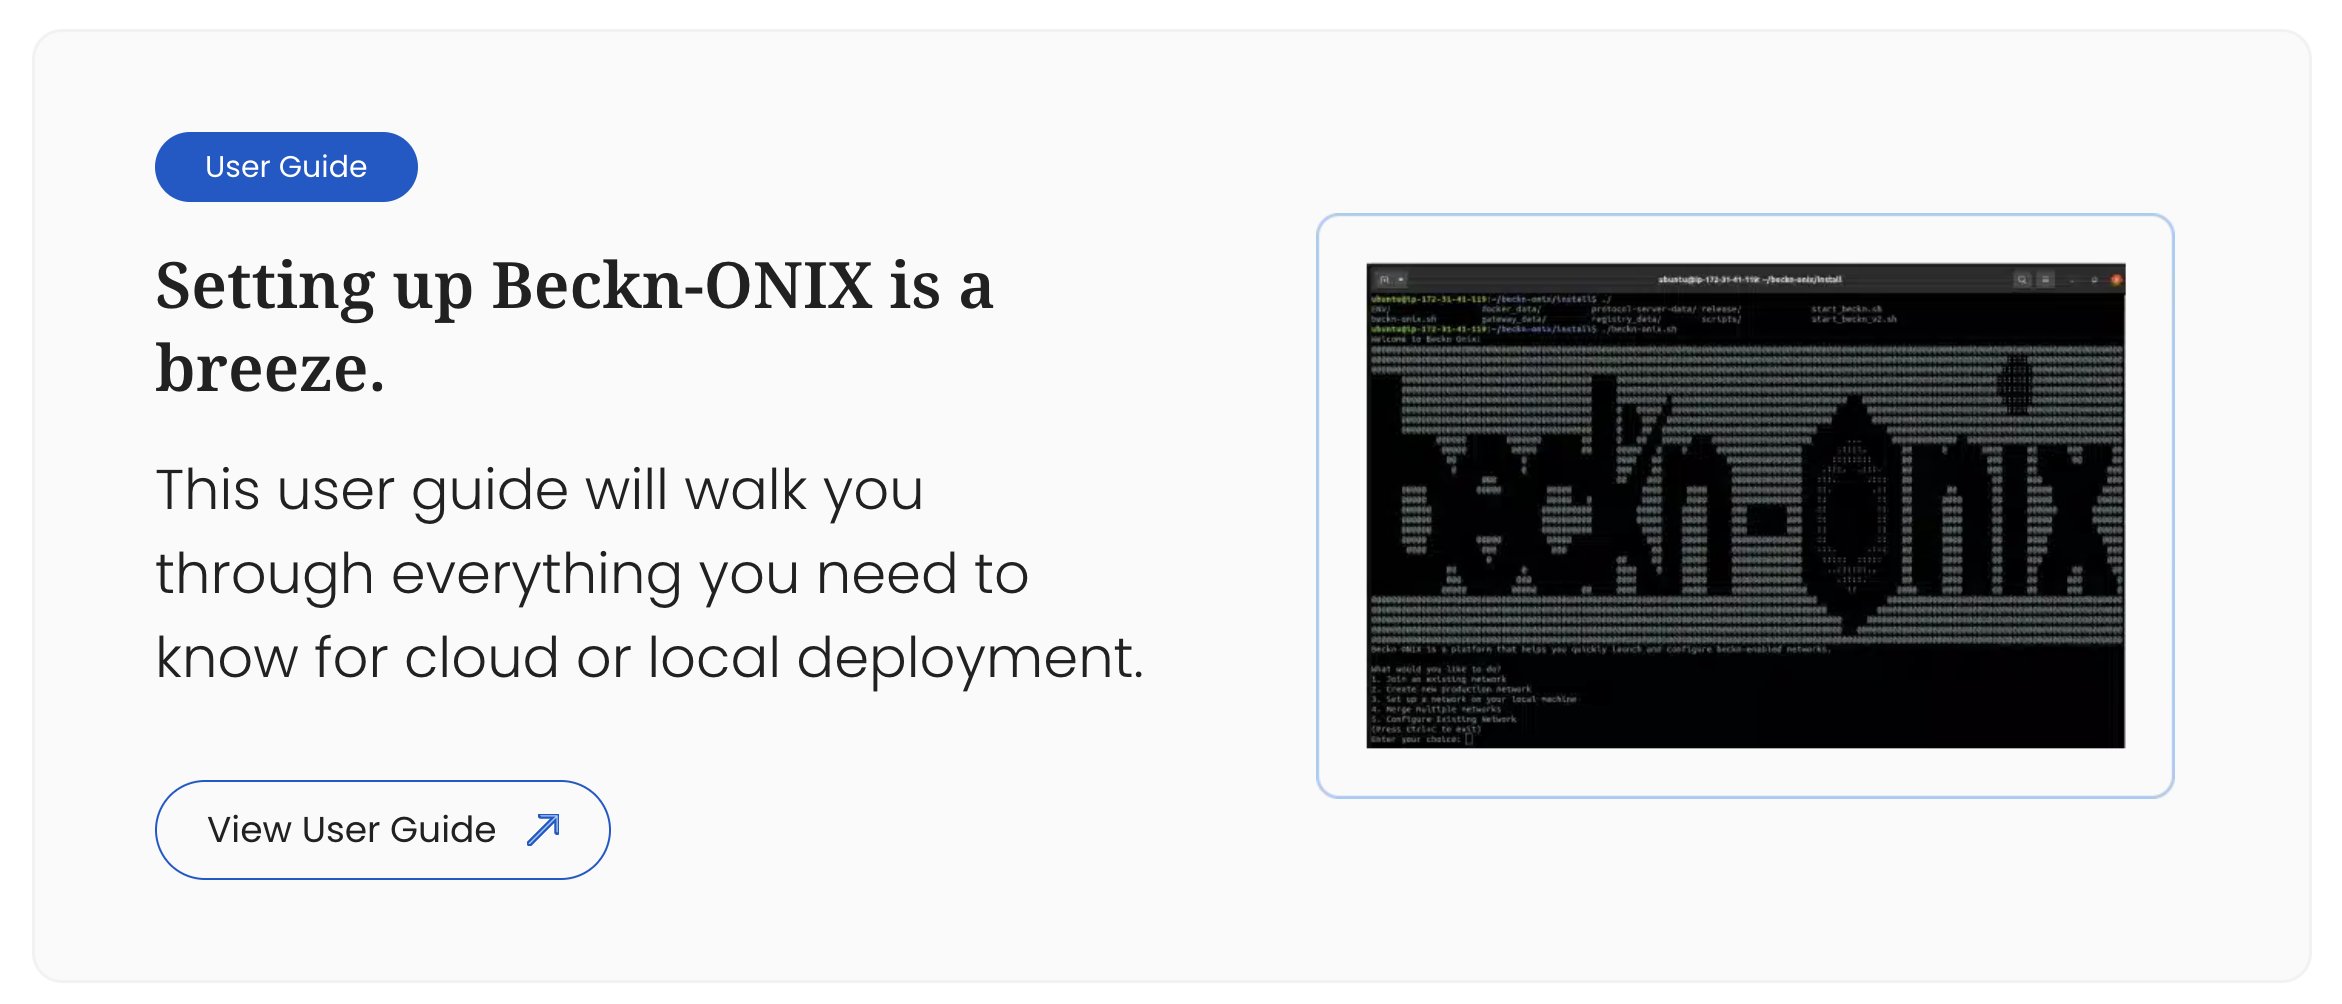
\includegraphics[width=0.8\textwidth]{Images/Beckn_Onix.png}
    \caption{Beckn-ONIX description. Screenshot taken from \cite{beckn_onix}}
    \label{fig:beckn_onix_picture}
\end{figure}

It is marketed as a rapid deployment tool, allowing users to have a functional network in minutes, which is what made us believe we could create a fully functional food ordering network. As previously mentioned, this unfortunately was not the case. We will discuss the issues related to Beckn-ONIX deployment in further detail in Section~\ref{second_sprint}
\subsection{API specifications}
The objective of the first sprint was to familiarize ourselves with the Beckn Protocol—its architecture, ecosystem, and potential applications—particularly in relation to our envisioned decentralized food delivery platform in Copenhagen. We aimed to understand how the protocol enables server communication, the structure of API endpoints, and what components are required for a functioning network.

Our research was primarily based on written and video documentation provided by Beckn. Fortunately, Beckn has a strong presence on YouTube, especially through a playlist titled Tech Overview containing 14 videos where Ravi Prakash, Head of Architecture and Technology Ecosystem at FIDE (formerly Beckn Foundation), dives into the technical aspects of the protocol.

These videos were especially helpful in building a foundational understanding of the protocol, including how the APIs are structured and how they fit into a typical economic transaction. The APIs are designed to work sequentially—from discovery to fulfillment—and while not every transaction uses all 10 APIs, the protocol’s open and extensible nature allows for additional APIs to be introduced if needed.

\begin{figure}[h]
\centering
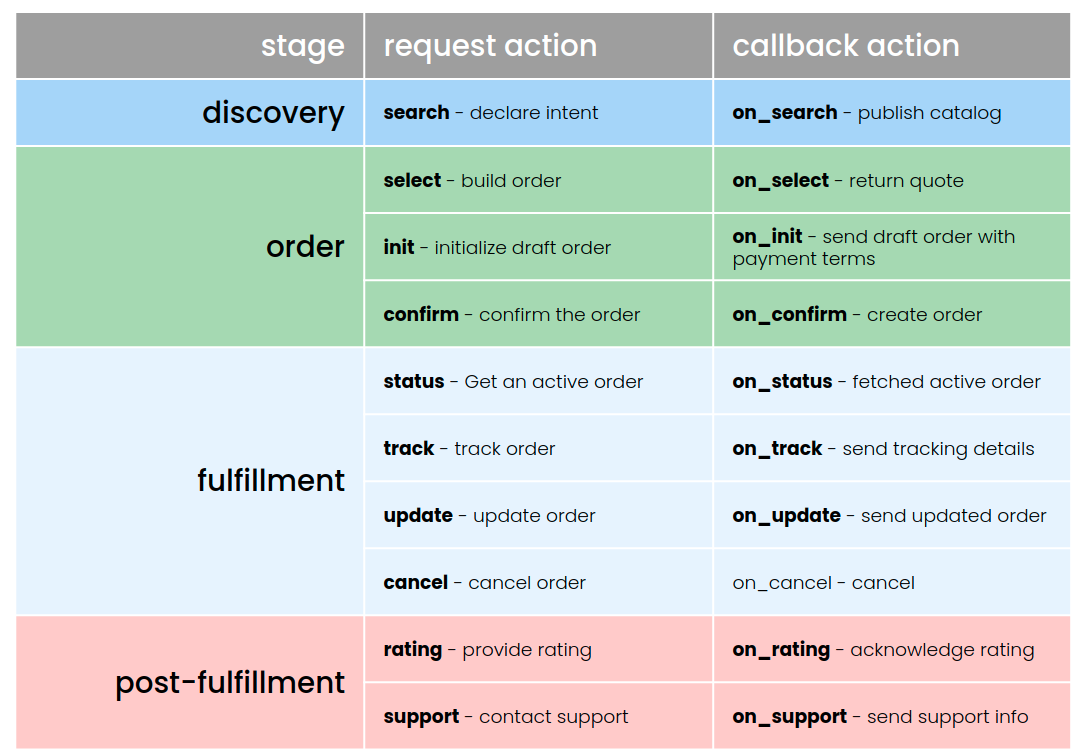
\includegraphics[width=0.5\textwidth]{Images/beck_api_overview.png}
\caption{Overview of the Beckn APIs}
\label{fig:beckn_api_overview}
\end{figure}
\subsection{Cloud Structure}
In one of the videos, Ravi Prakash explains how these APIs can be applied to any buyer/seller interaction. This flexibility is part of what makes Beckn sector-agnostic and suitable for a wide range of domains—from mobility to commerce.

\begin{figure}[h!]
\centering
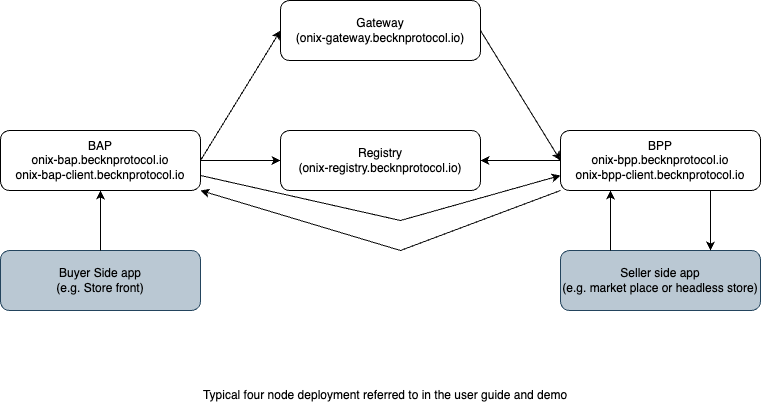
\includegraphics[width=0.8\textwidth]{Images/sample_deployment.png}
\caption{Sample deployment of Beckn-ONIX}
\label{fig:sample_deployment}
\end{figure}

We also examined the sample deployment diagram provided in the Beckn-ONIX documentation. It shows the four core servers—Registry, Gateway, BAP, and BPP—but also includes buyer and seller side apps. These were only mentioned in this diagram and not documented elsewhere, which led to some frustration. There were no reference implementations, and the step involving these apps was entirely skipped in the official \href{https://drive.google.com/file/d/1PfdhIpq-Qo6sDy0wAnO0zllCMGX718FW/view}{Beckn-ONIX CLI Setup video}. Given that these applications are where most of the domain-specific business logic lives, it took us quite a while to figure out how to simulate a full transaction.\newpage

\begin{figure}[h]
\centering
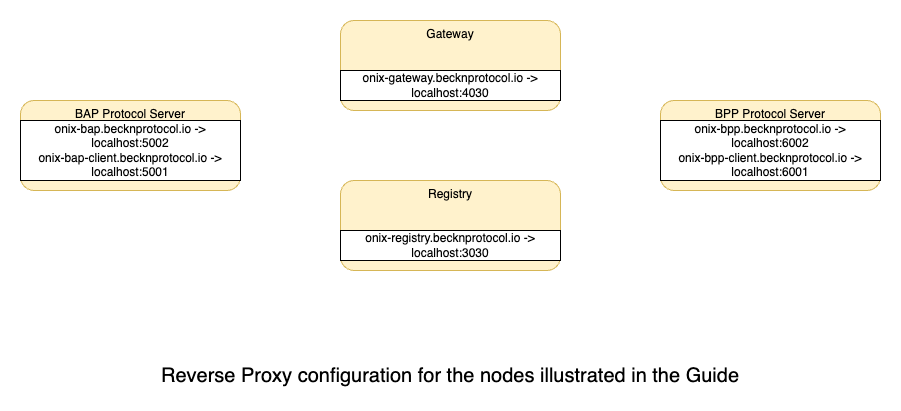
\includegraphics[width=0.8\textwidth]{Images/reverse_proxy_configuration.png}
\caption{Reverse Proxy Configuration required for Beckn-ONIX}
\label{fig:reverse_proxy_config}
\end{figure}

We did, however, find helpful information regarding reverse proxy configuration and subdomain setup. As shown above, we used this diagram as a guide to configure DNS records and match the required subdomain structure for each component.